\documentclass[12pt]{article}   % use documentclass amsart too if you want
\usepackage{amsmath,amsthm,amssymb}
\usepackage[margin=1in]{geometry}
\usepackage{color}
\usepackage{hyperref}
\usepackage{graphicx}
\usepackage{fancyhdr} % COMMENT THIS OUT TO TURN OFF FANCY HEADERS
\usepackage{verbatim}

\hypersetup{
  colorlinks= true, %Colours links instead of ugly boxes
  urlcolor   = blue, %Colour for external hyperlinks
  linkcolor  = blue, %Colour of internal links
  citecolor  = blue %Colour of citations
}





\newtheorem{theorem}[equation]{Theorem}
\newtheorem{lemma}[equation]{Lemma}
\newtheorem{corollary}[equation]{Corollary}
\theoremstyle{definition}
\newtheorem{exercise}[equation]{Exercise}

\newtheorem{example}[equation]{Example}
\newtheorem{definition}[equation]{Definition}
\newtheorem{question}[equation]{Question}
\newtheorem{remark}[equation]{Remark}

\numberwithin{equation}{section}

%@@@@@@@@@@@@@@@@@@@@@@@@@@@@@@@@@@@@@@@@@@@@@@@@@@@@@@@@@@@@@@@@@@@@@@@@@@@@@@@@@@@@@@@@@

\begin{document}
\parskip10pt
\parindent0pt
\baselineskip15pt


\title{APPM 2360 PROJECT 3: THE LOTKA-VOLTERRA PREDATOR PREY MODEL}
\author{Ethan Burkley (section 251), \\ Davis Landry (section 213), Max Morgan (section 244) \\ Jonathan Kish}


\pagestyle{fancy}
\renewcommand{\sectionmark}[1]{\markright{#1}{}}

\fancyhf{}

\rhead{\fancyplain{}{\thepage}} % predefined ()
\lhead{\fancyplain{}{\rightmark }} % 1. sectionname, 1.1 subsection name etc
%\cfoot{\fancyplain{}{\thepage}}

\maketitle

%@@@@@@@@@@@@@@@@@@@@@@@@@@@@@@@@@@@@@@@@@@@@@@@@@@@@@@@@@@@@@@@@@@@@@@@@@@@@@@@@@@@@@@@@@
\newpage
\lhead{Burkley, Landry, Morgan Project 3}
\setcounter{page}{2}

\section{Introduction} \label{APPM2360proj01sec01}
\quad Understanding the growth of a population is a complex challenge as population dynamics depend on a large number of factors such as fertility, size, and available resources. Understanding the growth of a population becomes more complicated when observing the biological system of two interacting species. There are many ways to model the relationship between the populations of a species of predator and prey. The populations of predators and prey are interdependent, however the size of one population causes spikes or dips in the other. Beyond just the size of the species' populations, there are many external factors that can influence the growth of these species. Including these into the model results in more accurate, yet more complex, models. More intricate models take into account factors found in populations such as carrying capacity and migration in order to better predict the future growth or decline of populations. The Lotka-Volterra model incorporates observational data of a species' growth and the rate of interactions between species in order to understand the dynamics of population of predators and prey. 

%@@@@@@@@@@@@@@@@@@@@@@@@@@@@@@@@@@@@@@@@@@@@@@@@@@@@@@@@@@@@@@@@@@@@@@@@@@@@@@@@@@@@@@@@
\setcounter{page}{1}
\section{Background} \label{APPM2360proj01sec01}
\quad A simplified population growth model assumes that the growth rate of the population $\frac{dP}{dt}$ is proportional to the current size of the of population $P$. This yields the differential equation $\frac{dP}{dt}=rP$, where $r$ is the intrinsic growth rate of the population. However, the model must be adjusted when considering the dynamics of a predator species interacting with a prey species. Both the populations will still grow proportionally to their size, but now the size of the other population must also be taken into consideration. The predator species population, with morality rate $a$, is supported by interactions with the prey species. The constant $b$ represents the reproduction rate of predator per prey. Therefore the predator population grows according to the following differential equation, 

\begin{equation}
  %
  \frac{dx_1}{dt} = -ax_1 + bx_1x_2 ,\ x_1(0) = x_{1,0}\\
  \label{eq:1}
  %
\end{equation}
where $x_{1,0}$ is the experimentally observed initial size of predator population. 

\quad The prey population grows according to the simplified population growth model, where the population growth rate is proportional to the population size. The constant $c$ represents the reproduction rate of the prey. Because the predator population hunts prey, population is negatively impacted by these interactions. The constant $d$ mortality rate of predator per prey. Therefore the prey population grows according to the following differential equation,
\begin{equation}
  %
  \frac{dx_2}{dt} = cx_1 - dx_1x_2 ,\ x_2(0) = x_{2,0} 
  \label{eq:2}
  %
\end{equation}

where $x_{2,0}$ is the experimentally observed initial size of prey population. 

\quad The Lotka-Volterra predator prey model uses the coupled system of differential equations to describe the dynamics of the two species' populations. The function $x_1(t)$ describes the size of the predator population with respect to time and the function $x_2(t)$ describes the prey population with respect to time. 

%@@@@@@@@@@@@@@@@@@@@@@@@@@@@@@@@@@@@@@@@@@@@@@@@@@@@@@@@@@@@@@@@@@@@@@@@@@@@@@@@@@@@@@@@
\setcounter{page}{2}
\section{Problem Statement} \label{APPM2360proj01sec01}
\quad The animal kingdom faces an ongoing biotic crisis, with a widespread and rapid decrease in the biodiversity on Earth due to human activity. Human influence has drastically reshaped the natural landscape, altering every aspect of the environment. Everything from animal migration patterns to food sources to seasonal breeding grounds have been impacted by human activity. This biotic crisis event has been labeled as the Holocene Extinction.

\quad Faced with this crisis, it is vital understand how these aspects of human influence alter the dynamics of animal populations. This investigation aims to understand how the dynamics of a competing predator and prey population can be modeled in the scope of both altered migration patterns and ecosystem carrying capacities.      

 



%@@@@@@@@@@@@@@@@@@@@@@@@@@@@@@@@@@@@@@@@@@@@@@@@@@@@@@@@@@@@@@@@@@@@@@@@@@@@@@@@@@@@@@@@
\setcounter{page}{2}
\section{Calculations and Results} \label{APPM2360proj01sec01} 

From here, the horizontal and vertical nullclines are determined by setting the $\frac{dx_1}{dt}$ and $\frac{dx_2}{dt}$ equal to zero. Conceptually, when $\frac{dx_1}{dt}$ is equal to 0, there is no change along the horizontal axis and when $\frac{dx_2}{dt}$ is equal to 0, there is no change along the vertical axis. 
\begin{align*}
  & \frac{dx_1}{dt} = \frac{dx_2}{dt} = 0
\end{align*}

Therefore the nullclines of equation (\ref{eq:1}) are the vertical nullclines of the system. The vertical nullcines are,
\begin{align*}
  %
  0 & =  -ax_1 + bx_1x_2 \\
  %  
  & = x_1(-a + bx_2) \\
  %
  x_1 &= 0, \ x_2 = \frac{a}{b}  
  %
\end{align*}
And the nullclines of equation (\ref{eq:2}) are the horizontal nullclines of the system. The horizontal nullclines are, 
\begin{align*}
  %
  0 & = cx_2 - dx_1x_2 \\  
  %
  & =  x_2(c - dx_1) \\
  %
  x_2 &= 0, \ x_1 = \frac{c}{d} 
\end{align*}

The two-dimensional system of autonomous, first order differential equations can be written in matrix vector form as a vector valued function, 
\begin{align*} 
  \textbf{x}'(t) 
  = 
  \begin{bmatrix}
    -ax_1 + bx_1x_2\\
    cx_2 - dx_1x_2\\
  \end{bmatrix}
\end{align*}

The Jacobian matrix for this system is given by the partial derivatives of (\ref{eq:1}) and (\ref{eq:2}).
\begin{align*} 
  J 
  =
  \begin{bmatrix}
    \frac{\partial{x'_1}}{\partial{x_1}} & \frac{\partial{x'_1}}{\partial{x_2}}\\
    \frac{\partial{x'_2}}{\partial{x_1}} &  \frac{\partial{x'_2}}{\partial{x_2}}\\
  \end{bmatrix}
  =
  \begin{bmatrix}
    -a+bx_2 & bx_1\\
    -dx_2 & c-dx_1\\
  \end{bmatrix}
\end{align*}

\quad Now,the stability of the equilibrium solutions for this system of differential equations can be determined by using the eigenvalues of the Jacobian matrix. If the Jocobian matrix's eigenvalues have a negative real part when evaluated at the equilibrium point, then the equilibrium is asymptotically stable. If the at least one of the eigenvalues has a positive real part, the equilibrium is unstable. And finally, if an eigenvalue of the Jacobian has a eigenvalue with a real part equal to zero, then the equilibrium point is neutrally stable. The Equilibrium points are at the points of intersection of a vertical nullcline and the horizontal nullcline. The vertical and horizontal nullclines intersect at $(0,0)$ and $(\frac{c}{d},\frac{a}{b})$.  

For $J$ evaluated at the equilibrium point $(0,0)$ the eigenvalues are $\lambda=-a,\ c$, which is unstable.
\begin{align*}
  \begin{vmatrix}
    -a-\lambda &0\\
    0& c-\lambda\\
  \end{vmatrix}
  =(-a-\lambda)(c-\lambda)
\end{align*}

For $J$ evaluated at the equilibrium point $(\frac{c}{d},\frac{a}{b})$ the eigenvalues are  $\lambda=\pm i\sqrt{ac}$, which is neutrally stable.
\begin{align*}
  \begin{vmatrix}
    0-\lambda & \frac{bc}{d}\\
    \frac{-da}{b} & 0-\lambda\\
  \end{vmatrix}
  =\lambda^2+ac
\end{align*}

\quad The physical interpretation of $(0,0)$ being unstable make sense in the context of this model because if any prey existed in this system, then the prey population would begin to grow and move away from the equilibrium point. Even though if one predator existed and died out, returning the system to the equilibrium point the equilibrium, is still unstable. 

\quad The point $(\frac{c}{d},\frac{a}{b})$ is neutrally stable which means that once there, the two populations will oscillate around that point. As the predator species grows, there will by more interactions with the prey species. This will have the effect of decreasing the size of the prey population as more predators hunt for food. A smaller prey population will in turn decrease the predator population by causing a food shortage. This decrease in the predator population ultimately allows the prey population to rebound and increase again. This balanced cycle repeats as time moves forward, as seen in \autoref{fig:dirfield}. 

\begin{figure} [h] 
  \centering
  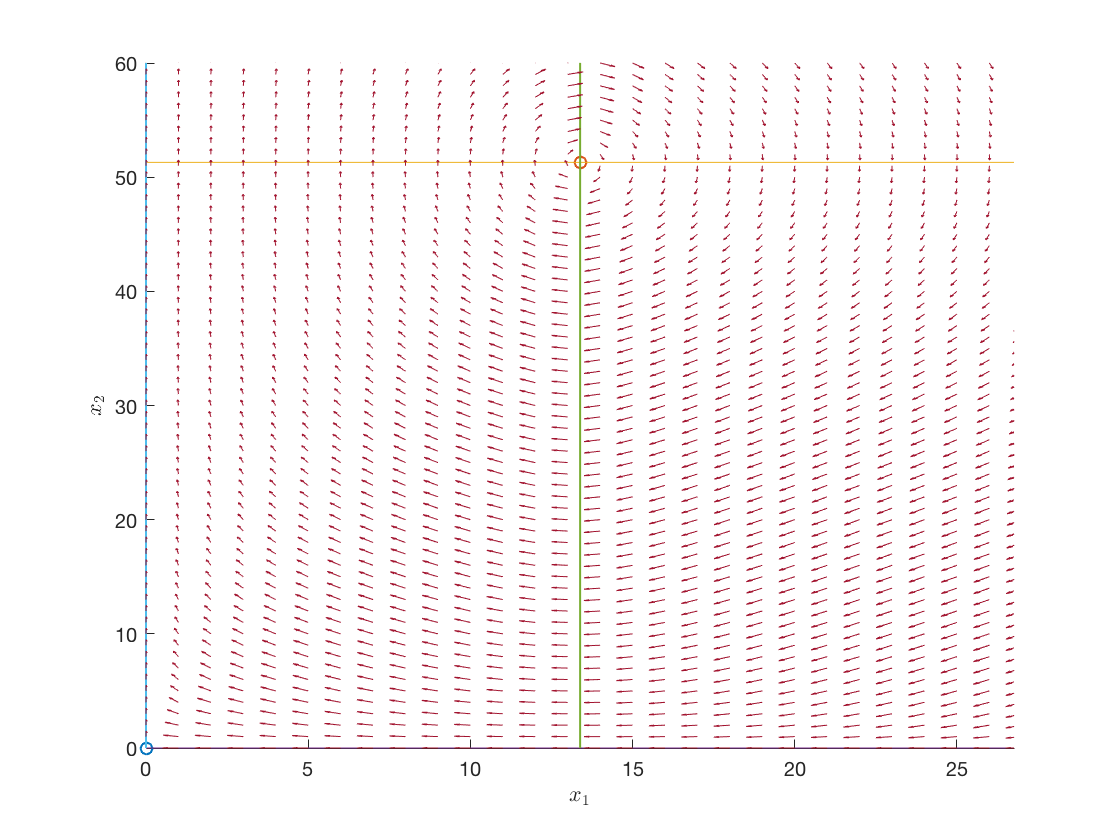
\includegraphics[width=15cm]{images/dirfield.png}
  \caption{Direction Field Plot}
  \label{fig:dirfield}
\end{figure}

\quad So far, the population model has been based off the assumption that the population grows exponentially without bound. However, in reality many aspects of the environment will limit the size of the populations. These population have a carrying capacity or a number of individuals the ecosystem can feasibly support. To reflect this, model must be altered to include this parameter.    
\begin{equation}
  \frac{dx_1}{dt} = -ax_1 + bx_1x_2
  \label{eq:4}
\end{equation}
\begin{equation}
  \frac{dx_2}{dt}= cx_1(1-kx_2) - dx_1x_2 
  \label{eq:5}
\end{equation}

\quad The physical meaning of parameter $k$ in (\ref{eq:5}) is the value of carrying capacity over one, therefore the units of $k$ are $prey^{-1}$.  The equilibrium solutions can be found when both (\ref{eq:4}) and (\ref{eq:5}) are equal to zero.  Solving for this gives,

\begin{align*}
  \frac{dx_1}{dt} =0= -ax_1 + bx_1x_2\\
  0=x_1(-a+bx_2)\\
  x_1=0,\ x_2=\frac{a}{b}\\
  \frac{dx_2}{dt}=0= cx_2(1-kx_2) - dx_1x_2\\
  0=x_2[c(1-kx_2)-dx_1]\\
  x_2=0,\ x_2=\frac{c-dx_1}{ck}
\end{align*}

\quad Therefore there are equilibrium points at $(0,0)$, $(0,\frac{c}{d})$, and if $k<\frac{b}{a}$ then there is also an equilibrium solution at $(\frac{a}{b},\frac{c(b-k)}{bd})$. $k$ must be less than $\frac{b}{a}$ because if it is not then that intersection of nullclines happens at a negative value of $x_1$ and is therefore unphysical in this problem.

\quad When (\ref{eq:4}) and (\ref{eq:5}) are solved numerically with ode45 where $k=0.001$ the resulting plot of $x_1 vs x_2$ is shown in \autoref{fig:circ001}.  These solutions show both periodic and asymptotic behavior. The plot cycles between periods of a low predator population with a high prey population and periods of a high predator population with a low prey population. 

\quad When (\ref{eq:4}) and (\ref{eq:5}) are solved numerically with ode45 where $k=0.02$ the resulting plot of $x_1 vs x_2$ is shown in \autoref{fig:circ02}.  These solutions show periodic behavior. The plot cycles between periods of a low predator population with a high prey population and periods of a high predator population with a low prey population. 

\begin{figure} [h] 
  \centering
  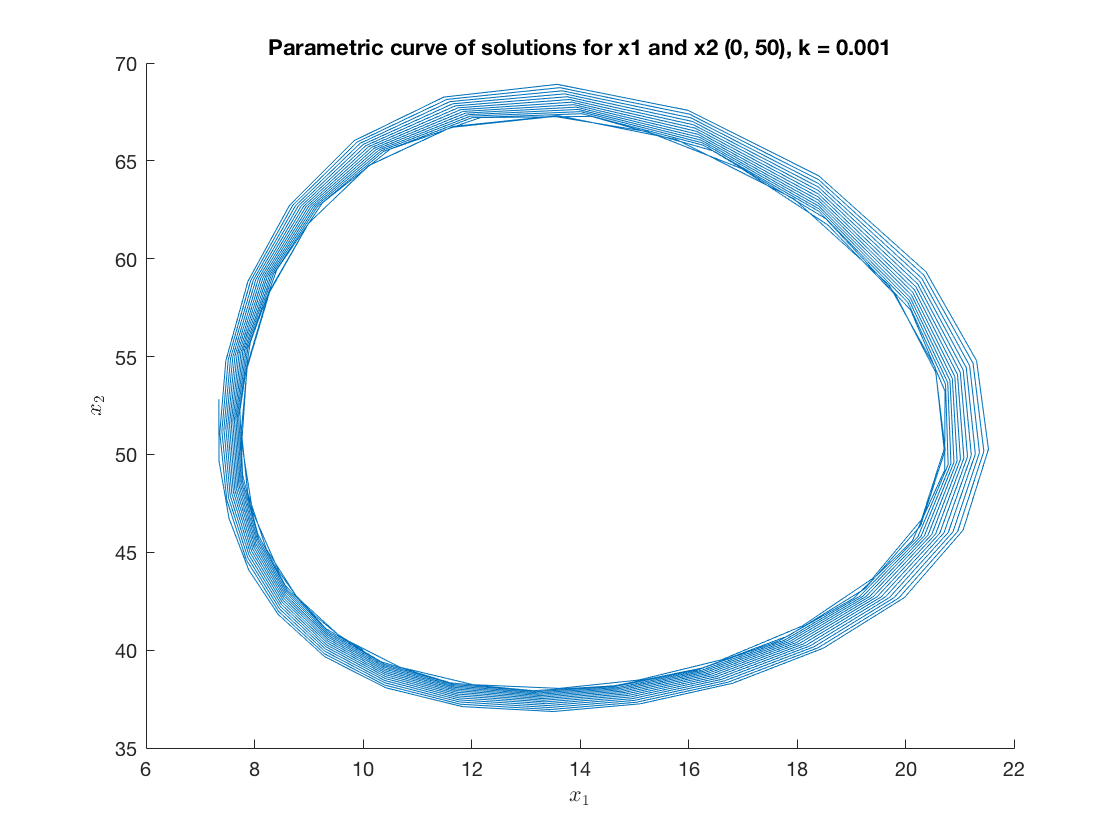
\includegraphics[width=10cm]{images/circ001.png}
  \caption{Plot of Population Oscillations with $k=0.001$}
  \label{fig:circ001}
\end{figure}

\begin{figure} [h] 
  \centering
    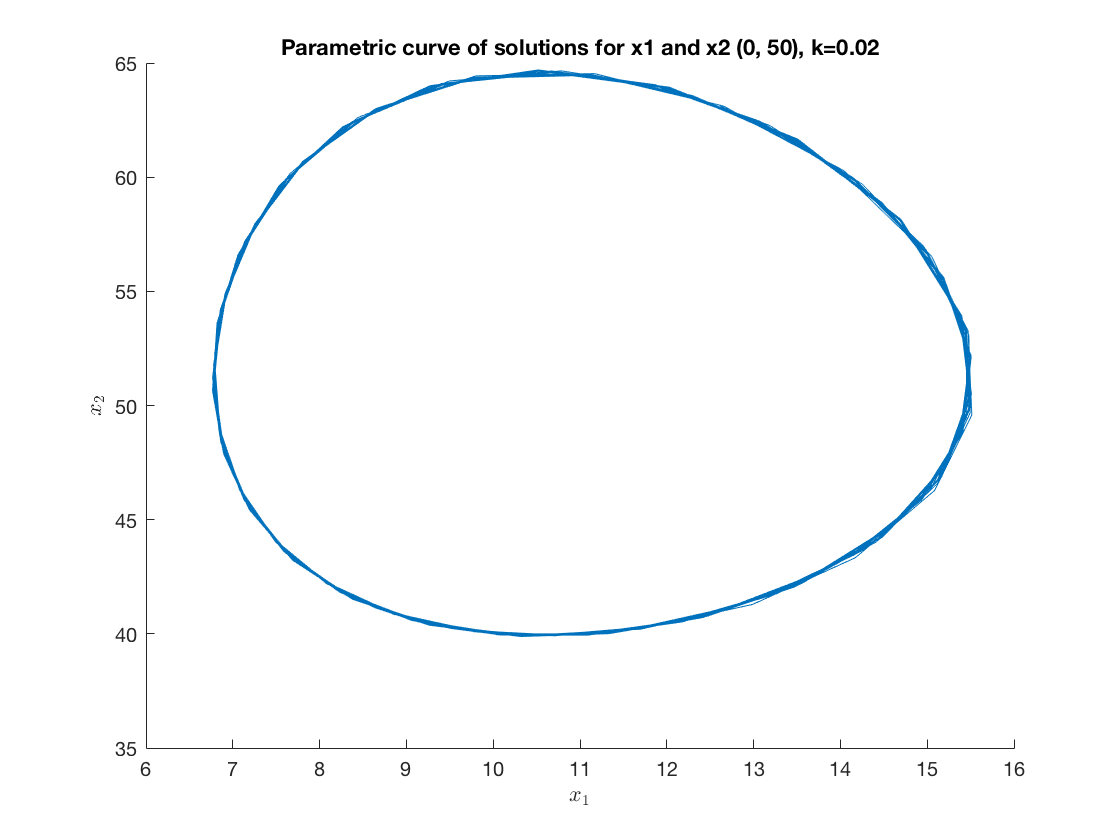
\includegraphics[width=10cm]{images/circ02.png}
  \caption{Plot of Population Oscillations with $k=0.02$}
  \label{fig:circ02}
\end{figure}

\quad The structure of these two solutions are very different, as they model different ecosystems capable of supporting different sized populations. In \autoref{fig:cir001}, the

%@@@@@@@@@@@@@@@@@@@@@@@@@@@@@@@@@@@@@@@@@@@@@@@@@@@@@@@@@@@@@@@@@@@@@@@@@@@@@@@@@@@@@@@@
\newpage
\setcounter{page}{4}
\section{Conclusion} \label{APPM2360proj01sec01}


%@@@@@@@@@@@@@@@@@@@@@@@@@@@@@@@@@@@@@@@@@@@@@@@@@@@@@@@@@@@@@@@@@@@@@@@@@@@@@@@@@@@@@@@@
\newpage
\setcounter{page}{7}
\section{Appendix} \label{APPM2360proj01sec01}

\end{document} 
